\documentclass[12pt,dvipsnames]{article}
 \usepackage[margin=1in]{geometry} 
\usepackage{amsmath,amsthm,amssymb,amsfonts}
 \usepackage{xcolor}
\newcommand{\N}{\mathbb{N}}
\newcommand{\Z}{\mathbb{Z}}
 \usepackage{graphicx,latexsym,amssymb}
 \usepackage{subcaption}
 \usepackage{parskip}
 \usepackage{epsfig}
 \usepackage{listings}
\usepackage{xcolor}
\usepackage{algpseudocode}
\usepackage{algorithm}
\usepackage{listings}
\usepackage{xcolor}
\usepackage{breqn}
\usepackage{mathtools}
\usepackage[english]{babel}
\usepackage{amsthm}
\newcommand\norm[1]{\left\lVert#1\right\rVert}
\newcommand\normx[1]{\left\Vert#1\right\Vert}
\DeclarePairedDelimiter\abs{\lvert}{\rvert}
\usepackage{amssymb}
\usepackage{booktabs}
\newtheorem{theorem}{Theorem}[section]
\newtheorem{claim}[theorem]{Claim}
%\usepackage{mcode}
% Syntax: \colorboxed[<color model>]{<color specification>}{<math formula>}
\newcommand*{\colorboxed}{}
\def\colorboxed#1#{%
  \colorboxedAux{#1}%
}
\newcommand*{\colorboxedAux}[3]{%
  % #1: optional argument for color model
  % #2: color specification
  % #3: formula
  \begingroup
    \colorlet{cb@saved}{.}%
    \color#1{#2}%
    \boxed{%
      \color{cb@saved}%
      #3%
    }%
  \endgroup
}
\usepackage{epsfig}
\newenvironment{problem}[2][Problem]{\begin{trivlist}
\item[\hskip \labelsep {\bfseries #1}\hskip \labelsep {\bfseries #2.}]}{\end{trivlist}}
\lstset { %
    language=C++,
    backgroundcolor=\color{black!5}, % set backgroundcolor
    basicstyle=\footnotesize,% basic font setting
}
%If you want to title your bold things something different just make another thing exactly like this but replace "problem" with the name of the thing you want, like theorem or lemma or whatever
\algdef{SE}% flags used internally to indicate we're defining a new block statement
[STRUCT]% new block type, not to be confused with loops or if-statements
{Struct}% "\Struct{name}" will indicate the start of the struct declaration
{EndStruct}% "\EndStruct" ends the block indent
[1]% There is one argument, which is the name of the data structure
{\textbf{struct} \textsc{#1}}% typesetting of the start of a struct
{\textbf{end struct}}% typesetting the end of the struct

\newcommand{\an}[1]{{\leavevmode\color{BrickRed}{#1}}}
\begin{document}
\title{Project 2: Spectral and finite volume methods}
\author{Gaurav Dhir}
\maketitle
\section{Solution 1}
We consider the Fourier Galerkin solution to the problem stated as Equation \ref{eq:Q1_problem} in the following subsections.
\begin{equation}
\begin{aligned}
& u_t + sin(2 \pi x)u_x = \frac{1}{2}u_{xx} \\
& u(x, 0) = sin( 2 \pi x ), x \in [0, 1], t > 0
\end{aligned}
\label{eq:Q1_problem}
\end{equation}
For the purposes of notational convenience, we represent the Partial Differential Equation (PDE) in the form described below:
\begin{equation}
    \begin{aligned}
        & u_t = R(u) = L(u) + P(u) \\
        & where \quad L(u) = \frac{1}{2}u_{xx} \quad and \quad P(u) = -sin(2 \pi x)u_x
    \end{aligned}
\label{eq:simplified}
\end{equation}
\subsection{(a)}
It is possible to arrive at a Semi-Discrete formulation for the Fourier Galerkin scheme for Equation \ref{eq:Q1_problem} in multiple ways.  The approaches can be summarized as the following:
\begin{itemize}
    \item Develop an appropriate formulation for the Fourier Basis Functions $\phi_k(x)$ where $\abs{k} \leq N$ such that the set of basis functions $\{ \phi_k(x) \}_{k = -N/2}^{N/2}$ are orthonormal with respect to the inner product defined as $<u, v> = \int_0^1 u(x) \overline{v(x)} dx$. 
      \an{I guess above you mean $|k| \leq N/2$ instead of $|k| \leq N$.}
      The set of Fourier Basis functions must also satisfy $\phi_k(x + 1) = \phi_k(x)$ for all $\abs{k} \leq N$ to ensure periodicity.
    \item Define a mapping from the interval $[0, 1]$ to $[0, 2 \pi]$ using a coordinate transformation such that the new coordinate $y$ satisfies $y \in [0, 2 \pi]$. Transform Equation \ref{eq:Q1_problem} in terms of $y$ and denote $v(y, t) = u(x, t)$ as the new solution variable. Use the orthonormal basis function $\phi_k(y) = e^{i k y}/\sqrt{2 \pi}$. This approach has been used to describe the application of the Fourier-Galerkin Scheme in Chapter $2$, Section $2.3$ of Shen, Tang and Wang. 
\end{itemize}
We describe the complete solution using the first approach stated above.

We devise an orthonormal set of the Fourier Basis functions $\phi_k(x) = c_1 e^{ic_2 kx}$ where $c_1$ is a normalizing constant and $c_2$ is chosen to satisfy the periodicity condition $\phi_k(x + 1) = \phi_k(x)$ for all $k \in Z$. It is easy to observe that the choice of $c_2 = 2 \pi$ leads to $\phi_k(x + 1) = c_1 e^{i 2 \pi k (x + 1)} = c_1 e^{ i 2\pi k x } e^{i 2 \pi k} = \phi_k(x)$ since $e^{i 2 \pi k} = 1$ for all $k \in Z$. Furthermore, the orthonormality condition requires that $<\phi_k(x), \phi_k(x)> = 1$. We know that $<\phi_k(x), \phi_k(x)> = \int_{0}^{1} c_1 e^{i2 \pi kx} c_1 e^{-i2 \pi kx}dx = c_1^2$. Hence, we arrive at the condition $c_1 = 1$. As a result, our Fourier Basis functions take the form $ \phi_k(x) =  e^{i2 \pi kx}$.  
\an{The above is fine, but I would be ok if you just asserted $\phi_k = e^{2 \pi i k x}$.}

The Fourier Series Approximation of a function $u(x, t) \in L^2[0, 2 \pi )$ is given as $u(x, t) = \sum_{k = -\infty}^{\infty} \hat{u}_k(t) e^{ikx}$. To utilize the Fourier Galerkin Scheme with finite spatial discretization, we consider the use of a truncated Fourier series expansion with fixed number of modes $\abs{k} \leq N$. Since, a minimum of two points are required in the spatial domain to resolve the smallest wavelength, we use $M = 2N + 1$ points to discretize the spatial domain $[0, 1]$.

The truncated Fourier Series approximation $u(x, t) \approx P_N u(x, t) = u_N(x, t) = \sum_{\abs{k} \leq N} \hat{u}_k(t) e^{i2 \pi kx}$ is represented as a projection to the finite dimensional space $V_N = span\{ e^{i 2 \pi kx}, \abs{k} \leq N \}$. The dimension of this space is $2N + 1$.

We use the strong form weighted residual method to devise the Fourier Galerkin discretization of Equation \ref{eq:simplified} as stated in Equation \ref{strongformweighted}.
\begin{equation}
    \begin{aligned}
        & <(u_N)_t, v> = <R(u_N), v> = <L(u_N), v> + <P(u_N), v> \forall v \in V_N \\
        & where \quad V_N = span\{ \phi_k(x) = e^{i2 \pi kx}, \abs{k} \leq N \}
    \end{aligned}
    \label{strongformweighted}
\end{equation}

Consider the evaluation of the term $<L(u_N), v> = <(u_N)_{xx}/2, \phi_k(x)>$. We know that $ u_N(x, t) = \sum_{\abs{k} \leq N} \hat{u}_k(t) e^{i2 \pi kx}$. It is possible to differentiate the series term by term to obtain $(u_N)_{x}(x, t) = \sum_{\abs{k} \leq N} \hat{u}_k(t) (i 2 \pi k) e^{i2 \pi kx}$. Let $c_k = i2 \pi k$, then $(u_N)_{xx}(x, t) = \sum_{\abs{k} \leq N} \hat{u}_k(t) c_k^2 e^{i2 \pi kx}$. It is interesting to observe that $L(u_N)$ lies completely inside the space $V_N$. As a result, the truncation error for this term is $0$ as also illustrated in Hesthaven providing validation for the fact that the truncation error for linear constant coefficient spatial operators is identically zero. Due to orthonormality of the Fourier Basis functions, we can observe the following:
\begin{equation}
    <L(u_N), \phi_k(x)> =c_k^2 \hat{u}_k(t)/2
    \label{LuN}
\end{equation}
Consider now the evaluation of the term $<P(u_N), v> = <-sin(2 \pi x)(u_N)_x, v>$ or $<P(u_N), v> = <-sin(2 \pi x)(u_N)_x, \phi_k(x)>$. We know that $sin(2 \pi x) = (e^{i 2 \pi x} - e^{-i 2 \pi x})/(2i) = (\phi_1(x) - \phi_{-1}(x))/(2i)$. Also, $(u_N)_{x}(x, t) = \sum_{\abs{k} \leq N}  \hat{u}_k(t) c_k e^{i2 \pi kx}$. On using these identities, we obtain $P(u_N) = \sum_{\abs{k} \leq N} \hat{u}_k(t) c_k (\phi_{k + 1} - \phi_{k - 1})/(2i)$. It is interesting to observe that unlike the term $L(u_N)$, the term $P(u_N)$ does not completely lie in the space defined by $V_N$. On further simplification of this term assuming $\hat{u}_{N + 1} = \hat{u}_{-N - 1} = 0$ and using $l = k + 1$, $s = k  - 1$, we can observe the following:
\begin{equation}
    P(u_N) = \sum_{\abs{l} \leq N} \frac{ \hat{u}_{l - 1}(t) c_{l - 1} }{2i} \phi_l(x) - \sum_{\abs{s} \leq N} \frac{\hat{u}_{s + 1} c_{s + 1}}{2i} \phi_s(x) + \frac{ \hat{u}_{N} c_{N} \phi_{N + 1} - \hat{u}_{-N} c_{-N} \phi_{-N - 1} }{2i}. 
    \label{PuN}
\end{equation}
It is easy to observe that $P(u_N)$ has a finite projection on $\phi_{N + 1}$ and $\phi_{-N - 1}$. As a result, its projection on $P_N$ introduces a finite truncation error. This is also indicated in Chapter $3$ of Hesthaven stating finite truncation error for the projection of non linear spatial operators on the space defined by $V_N$. It is also easy to observe that the projection operation in the Fourier Galerkin scheme does not alias the truncation error components. On the other hand, the usage of interpolation operation will most possibly introduce a finite aliasing error by representing them within the basis defined by $V_N$.

Using Equation \ref{PuN}, it is now possible to evaluate $<P(u_N), \phi_k(x)>$ which is now given as the following:
\begin{equation}
\begin{aligned}
    & <P(u_N), \phi_k(x)> = \frac{\hat{u}_{k - 1} c_{k - 1}}{2i} - \frac{\hat{u}_{k + 1} c_{k + 1}}{2i} = \pi\left( \hat{u}_{k - 1}(k - 1) - \hat{u}_{k + 1}(k + 1)  \right) \\
    & where \quad \hat{u}_{N + 1} = \hat{u}_{-N - 1} = 0
\end{aligned}
\label{projection_of_PuN}
\end{equation}
Also, for the time dependent term, it is easy to observe the following:
\begin{equation}
    <(u_N)_t, \phi_k(x)> = \frac{d \hat{u}_k(t)}{dt}
    \label{timedep}
\end{equation}
Using Equations \ref{strongformweighted}, \ref{LuN} and \ref{PuN}, we arrive at the final semi discrete formulation for the Fourier Galerkin Scheme shown as the following:
\begin{equation}
\begin{aligned}
    & \frac{d \hat{u}_k(t)}{dt} = - 2 \pi^2 k^2 \hat{u}_k + \pi (k + 1) \hat{u}_{k + 1} - \pi (k - 1) \hat{u}_{k - 1} \\
    & where \quad \abs{k} \leq N
\end{aligned}
\label{semidiscrete}
\end{equation}
It is also possible to write the semidiscrete formulation as a system of equations. Assuming $\hat{U} = \{ \hat{u}_{-N}, \hat{u}_{-N + 1}, \ldots \hat{u}_k, \ldots \hat{u}_{N} \}$ we obtain $\hat{U}_t = A\hat{U}$ where the tridiagonal components of the matrix $A$ are given as $A_{k,k} = - 2 \pi^2 (k - N)^2$, $A_{k, k+ 1} = \pi (k - N + 1)$, $A_{k, k - 1} = -\pi (k - N - 1)$ for $k$ varying from $[0, 2N + 1)$ and $k \in Z$. Also, $A_{i, j} = 0$ for $\abs{i - j} \geq 2$.

\subsection{(b)}
Using the semidiscrete formulation as a system of equations $\hat{U}_t = A\hat{U}$, and diagonalizing the matrix $A$ in terms of its left and right eigenvectors, we can obtain an uncoupled system of equations. In other words, using $A = L \Lambda R$ where $\Lambda$, $L$ and $R$ denote the matrix of eigenvalues (which can be complex), the left and the right eigenvectors of $A$ respectively and using $\hat{U}_t = LW_t$, $\hat{U} = R^{-1} W$, we obtain, $W_t = \Lambda W$ where $W$ now denotes the components of this uncoupled system of equations since $\Lambda$ is a diagonal matrix composed of the eigenvalues of $A$ on its diagonal. 

Let $w_k$ denote a specific component of $W$ and $\lambda_k$ denote a specific eigenvalue of $A$. Then, we obtain an uncoupled system of equations described in Equation \ref{equncoupled}.
\begin{equation}
\begin{aligned}
    & \frac{dw_k}{dt} = \lambda_k w_k \\
    & where \quad k \in [0, 2N + 1) \quad and \quad k \in Z
\end{aligned}
    \label{equncoupled}
\end{equation}
Using the Forward scheme for the discretization of Equation \ref{equncoupled} with timestep $\Delta t$ and denoting superscript $n$ as representing the time level, we obtain Equation \ref{eqforwardeuler}.
\begin{equation}
    \begin{aligned}
       & w_k^{n + 1} = w_k^{n} + \lambda_k \Delta t w_k^n \\
       & or \quad w_k^{n + 1} = (1 + z_k) w_k^{n} \\
       & where \quad z = \lambda_k \Delta t
    \end{aligned}
\label{eqforwardeuler}
\end{equation}
An A stable scheme must ensure $\abs{ w_k^{n + 1} } \leq \abs{ w_k^n }$ for every value of $k$. Hence, it must be the case that $\abs{1 + z_k} \leq 1$ for every $k$. Assuming, $\Re(z_k) = a$ and $\Im(z_k) = b$, one obtains the condition $(1 + a)^2 + b^2 \leq 1$ or $a^2 + b^2 + 2a \leq 0$. Since, $\Delta t$ is always real, we obtain $\Delta t( \Re(\lambda_k)^2 + \Im(\lambda_k)^2  ) + 2 \Re(\lambda_k) \leq 0$. Since, $\abs{\lambda_k}^2 = \Re(\lambda_k)^2 + \Im(\lambda_k)^2$, we obtain the time stepping condition as shown in Equation \ref{timestepfeuler}.
\begin{equation}
    \Delta t \leq \frac{-2 \Re(\lambda_k)}{\abs{\lambda_k}^2} \quad \forall k \in [0, 2N + 1)
    \label{timestepfeuler}
\end{equation}
\begin{figure}
    \centering
    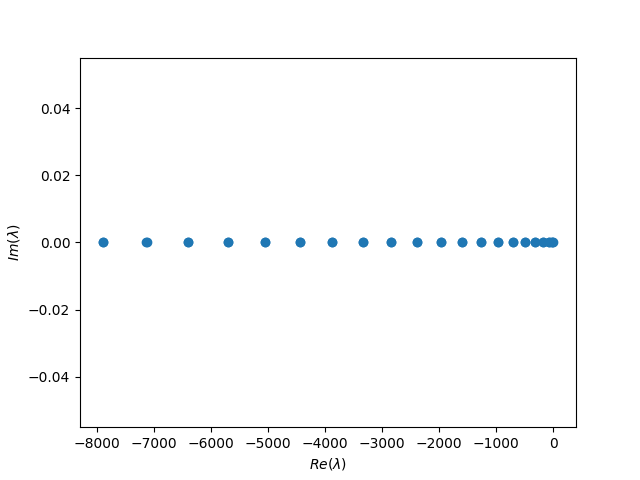
\includegraphics[width=10cm]{eigenplot_u_Q1.png}
    \caption{Eigenvalues of the matrix $A$ in the semidiscrete formulation for the Fourier Galerkin Scheme shown in Equation \ref{semidiscrete}}
    \label{eigenplot_Q1}
\end{figure}
The eigenvalues of the matrix $A$ are shown in Equation \ref{eigenplot_Q1}. It is found that the eigenvalues are all real and negative. Hence, the time stepping condition can be further simplified as $\Delta t \leq -2 / \lambda_k$ $\forall k \in [0, 2N + 1)$. Therefore, the most negative value of $\lambda_k$ decides the time stepping criteria given as $\Delta t \leq -2/min(\lambda_k)$.

The maximum possible timestep for the Forward Euler discretization of Equation \ref{semidiscrete} was plotted as a function of $N$ and can be observed in Figure \ref{timestep_restrict_Q1}. As seen in the figure, the timestep scales as $O(1/N^2)$. The slope of the linear curve in the plot was also calculated and was found to be exactly equal to $-2$.
\begin{figure}
    \centering
    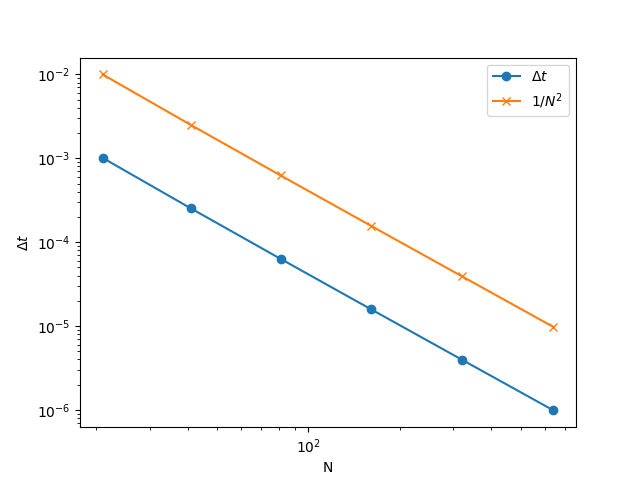
\includegraphics[width = 10cm]{dtvariation.png}
    \caption{Maximum Timestep restriction versus $N$ for the Forward Euler discretization of Equation \ref{semidiscrete} }
    \label{timestep_restrict_Q1}
\end{figure}

In order to analyze componentwise contributions to the time stepping restriction, the eigenvalues of the Fourier Galerkin discretization for the spatial operators $L$ and $P$ as stated in Equations \ref{LuN} and \ref{PuN} were calculated and the time stepping restrictions were calculated based on Equation \ref{timestepfeuler}. The plots for the timestep restrictions due to the eigenvalues of these spatial operators can be seen in Figure \ref{fig:componentwise_restriction}.
\begin{figure}
    \centering
    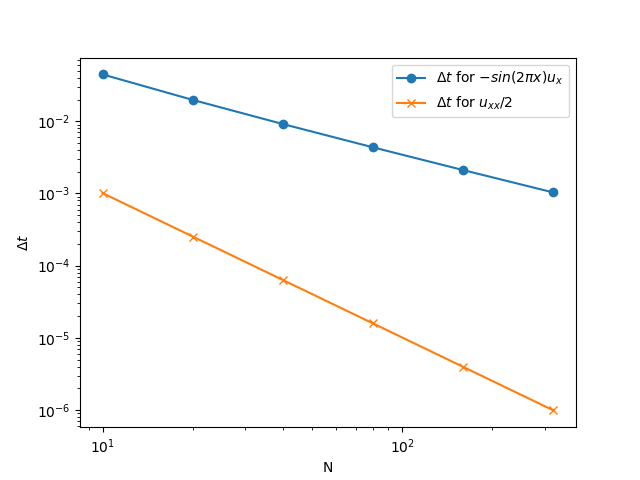
\includegraphics[width=10cm]{dtComponentwise_Q1.png}
    \caption{Componentwise restrictions to the time stepping criteria for the Forward Euler discretization plotted as a function of $N$}
    \label{fig:componentwise_restriction}
\end{figure}
As observed from the plot, it can be found that the term $u_{xx}/2$ enforces the most severe restrictions on the time stepping criteria. The slope of the curve corresponding to the time stepping restriction for $-sin(2 \pi x)u_x$ was calculated and was found to be equal to $-1.08$. On the other hand, the slope for the time stepping restriction for $u_{xx/2}$ was found to be equal to $-2$. The reasons can be attributed to the stiff behavior of the second derivative term $u_{xx}/2$ which makes the total computational time of the solver scale as $O(1/\Delta t) = O(N^2)$.  
\subsection{(c)}
Numerical implementation of the Fourier Galerkin scheme using any method requires the initial conditions to be calculated in the modal space of Fourier coefficients. The initial condition in the physical space is given as $u(x, 0) = sin(2 \pi x)$. One can either perform a Fourier transform of the initial conditions to calculate the Fourier Basis Coefficients or resort to analytical evaluation of these coefficients for simple cases. Since, $sin(2 \pi x) = (e^{i 2 \pi x} - e^{-i 2 \pi x})/(2i)$ the analytical formulation in the modal space can be found and is stated in Equation \ref{initialmodal}.
\begin{equation}
    \begin{aligned}
        & \hat{u}_{-1}(0) = \frac{-1}{2i}, \quad \hat{u}_{1}(0) = \frac{1}{2i} \\
        & and \quad \hat{u}_k(0) = 0 \quad \forall k \notin \{ -1, 1 \}
    \end{aligned}
    \label{initialmodal}
\end{equation}
\subsubsection{Crank Nicolson Formulation}
The Crank Nicolson scheme was used for the implicit formulation of the semi discrete formulation given as a system of ordinary differential equations $d \hat{U}/dt = A \hat{U}$. The Crank Nicolson scheme is stated in Equation \ref{cranknicolson}.
\begin{equation}
    \begin{aligned}
        & \hat{U}^{n + 1} = \hat{U}^n + \Delta t \left( \frac{A \hat{U}^{n + 1} + A \hat{U}^{n} }{2} \right) \\
        & or \quad \left( I - \frac{A \Delta t}{2} \right) \hat{U}^{n + 1} = \left( I + \frac{A \Delta t}{2} \right) \hat{U}^n \\
        & or \quad \hat{U}^{n + 1} = \left( I - \frac{A \Delta t}{2} \right)^{-1} \left( I + \frac{A \Delta t}{2} \right) \hat{U}^n
    \end{aligned}
    \label{cranknicolson}
\end{equation}
It can be easily observed that the term $\left( I - \frac{A \Delta t}{2} \right)^{-1} \left( I + \frac{A \Delta t}{2} \right)$ does not depend on $\hat{U}$. Hence, this term can be precalculated before the start of the solver. Let $G = \left( I - \frac{A \Delta t}{2} \right)^{-1} \left( I + \frac{A \Delta t}{2} \right)$. Assuming $\hat{U}_0$ stores the initial conditions, the solution at any time level $n$ can be simply calculated as $\hat{U}^n = G^n \hat{U_0}$ or by a series of matrix vector multiplications performed in a $for$ loop.
The stability criteria for the Crank Nicolson scheme includes the entire left half plane of the Argand Diagram of $z = \lambda \Delta t$. From Figure \ref{eigenplot_Q1}, it was observed that the eigenvalues of the matrix $A$ are all real and negative. Hence, the Crank Nicolson scheme is stable for the current problem.
\subsubsection{RK4 Formulation}
The $RK4$ scheme was used for the explicit time stepping formulation of the system of Ordinary Differential Equations $d\hat{U}/dt = A \hat{U}$. The $RK4$ scheme is stated in Equation \ref{eqRK4}.
\begin{equation}
    \begin{aligned}
        & \alpha^{(1)} = \Delta t A \hat{U^n} \\
        & \alpha^{(2)} = \Delta t A( \hat{U^n} +  \alpha^{(1)}/2 ) \\
        & \alpha^{(3)} = \Delta t A( \hat{U^n} +  \alpha^{(2)}/2 ) \\
        & \alpha^{(4)} = \Delta t A( \hat{U^n} +  \alpha^{(3)} ) \\
        & \hat{U}^{(n + 1)} = \hat{U^n} + \frac{1}{6} \left( \alpha^{(1)} + 2\alpha^{(2)} + 2\alpha^{(3)} + \alpha^{(4)} \right)
    \end{aligned}
    \label{eqRK4}
\end{equation}
The stability criteria for the $RK4$ scheme involves that the condition $1 + z_k + z_k^2/2 + z_k^3/6 + z_k^4/24 \leq 1$ be satisfied for every $z_k = \lambda_k \Delta t$ where $\lambda_k$ denotes the eigenvalue of the matrix $A$. Since, the eigenvalues of $A$ are all real, one obtains the condition, $1 + z_k/2 + z_k^2/6 + z_k^3/24 \leq 0$ to ensure stability. The equation $1 + z_k/2 + z_k^2/6 + z_k^3/24 \leq 0$ was solved and the maximum negative value that $z_k$ could take was found to be equal to $-2.7853$. Since the eigenvalues $\lambda_k$ are all negative, this leads to the condition $\Delta t \leq -2.7853/min(\lambda_k)$.
\subsubsection{Results and Discussion}
The results for both the explicit $RK4$ scheme and the implicit Crank Nicolson scheme for $N = 20$ were obtained and have been shown in Figure \ref{fig:q1solutioncomp}.
\begin{figure}
    \centering
    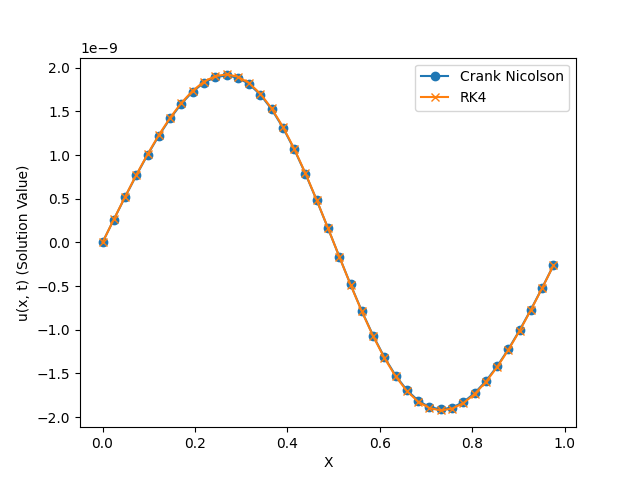
\includegraphics[width=10cm]{Q1SolutionComparisont=0.001.png}
    \caption{Solution plots for the RK4 and the Crank Nicolson Scheme at $t = 1.0$ and $N = 20$ \an{Since the solution values are so small, it's clear that I unfortunately chose the viscosity too large :(}}
    \label{fig:q1solutioncomp}
\end{figure}
The dissipative nature of the $u_{xx}/2$ term can be very easily observed from the plot since the initial solution value varying from $[-1, 1]$ dissipates to values ranging on the order of $1e-9$ at $t=1.0$. Furthermore, it is observed that the two solutions show excellent match despite the usage of different time steps for both the schemes. For the Crank Nicolson solution shown in Figure \ref{fig:q1solutioncomp}, a timestep of $0.00127$ was chosen while the maximum allowable timestep of $0.000352$ was used for the $RK4$ scheme. The unconditionally stable nature of the Crank Nicolson scheme allowed to take a timestep which was $3.59$ times greater than the timestep used for the $RK4$ scheme while still showing excellent match with the $RK4$ solution. 

Timing comparisons performed for the $RK4$ scheme and the Crank Nicolson scheme show a performance improvement by a factor of around $6$ for the Crank Nicolson scheme due to the larger allowable timestep. The performance improvements became more noticeable at higher values of $N$ despite the cost of a matrix inversion for the implicit Crank Nicolson scheme. It must also be noted that the current implementation of the RK4 scheme is inefficient and requires the usage of multiple matrix vector products. On the other hand, there is only one matrix vector product performed for the Crank Nicolson scheme per timestep after the initial computation of the matrix inverse. This also causes the RK4 scheme to take more time than expected. \an{I wouldn't call your RK4 implementation that inefficient. You generally can't circumvent the required number of matvec operations.}

Further analysis was performed by increasing the timestep value for the implicit Crank Nicolson scheme and comparing the obtained solution values with the explicit $RK4$ scheme. The results can be seen in Figure \ref{fig:CNTimestep}. Although the Crank Nicolson scheme shows stable behavior for these timestep values, the added stability comes at the cost of much higher dissipation of the solution values. Hence, although it might be possible to use very large timestep values for the implicit Crank Nicolson scheme, the obtained solution values might not be accurate. Furthermore, although, explicit schemes suffer from timestep limitations, for non linear and highly time accurate computations, the explicit schemes might provide faster solution values owing to no requirement of a matrix inversion.
\an{In this particular case the system defined by the Crank-Nicolson solver is tridiagonal, so inverting it is actually (asymptotically) just as inexpensive as computing a single vector dot product; so here if you optimize everything, it will still be the case that CN is much more efficient. (For example, your code computes a dense inverse for CN, which is technically not necessary, but is certainly the easiest thing to code.)}
\begin{figure}
\centering
    \subfloat[\centering $\Delta t_{CN} = 14 \times \Delta t_{RK4}$ ]{{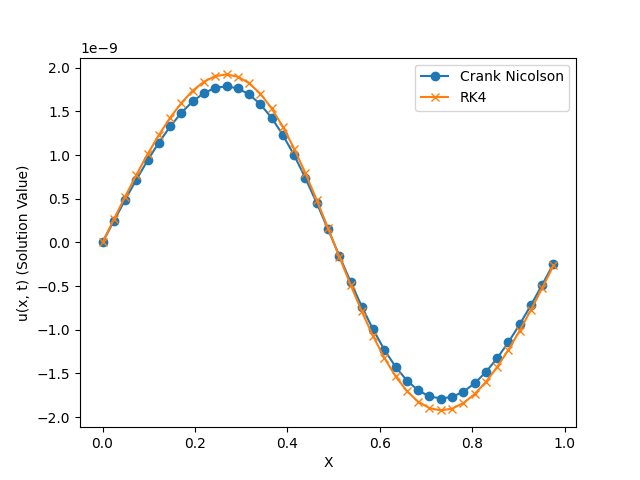
\includegraphics[width=8cm]{Q1SolutionComparisont=0.005.png} }}%
    \qquad
    \subfloat[\centering $\Delta t_{CN} = 71 \times \Delta t_{RK4}$ ]{{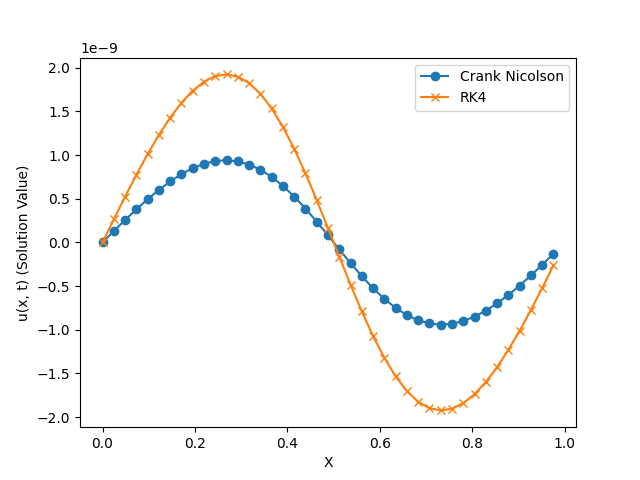
\includegraphics[width=8cm]{Q1SolutionComparisont=0.025.png} }}%
    \caption{Solution Comparison between the RK4 Scheme and the Implicit Crank Nicolson scheme for larger Crank Nicolson Time Steps}%
    \label{fig:CNTimestep}%
\end{figure}
\section{Solution 2}
We consider the solution to the problem stated as Equation \ref{eq:Q2_problem} in the following subsections.
\begin{equation}
\begin{aligned}
& u_t = R(u) = -u_{xxx} + 6uu_x \\
& u(x, 0) = -2sech^2(x), \quad x \in [-10, 10], \quad t > 0
\end{aligned}
\label{eq:Q2_problem}
\end{equation}
Let $M = 2N + 1$ represent the total number of points used in the spatial discretization of the domain $[-10, 10]$. Here, $N$ represents the value of the maximum wavenumber approximated in the truncated Fourier expansion of the solution variable $u$. In other words, $u_N(x, t) = \sum_{\abs{k} \leq N} \hat{u}_k(t) \phi_k(x)$ where $\phi_k(x)$ represents the individual Fourier Basis mode. It is well known that the Fourier expansion can be recast in the form of an interpolating trigonometric polynomial. In other words, the previous Fourier expansion is equivalent to the form $u(x, t) = \sum_{j = 0}^{M - 1} u_N(x_j, t) g_j(x)$ where $g_j(x)$ is the trigonometric lagrange interpolating polynomial.

It is possible to differentiate the Lagrange interpolating polynomial term by term to obtain the collocation representation for the derivatives $u_{xxx}$ and $u_x$. However, we resort to the use of performing differentiation in the modal space and then use the inverse Fourier transform to project the differentiated values back to physical space. Let $\Tilde{D}_3$ and $\Tilde{D}_1$ represent the differentiation matrices corresponding to the collocation discretization of $u_{xxx}$ and $u_x$ respectively. Furthermore, let $U$ represent the vector of point values corresponding to the solution variable $u(x, t)$. Then, the semi discrete formulation corresponding to the Fourier Collocation discretization of Equation \ref{eq:Q2_problem} has been described in Equation \ref{eq:Q2:explicit_collocation}.
\begin{equation}
\begin{aligned}
    U_t = -\Tilde{D}_3 U + 6U \odot \Tilde{D}_1 U
\end{aligned}
\label{eq:Q2:explicit_collocation}     
\end{equation}
\subsection{(a)}
Consider an explicit time stepping scheme for the solution of Equation \ref{eq:Q2:explicit_collocation}. The explicit schemes for the semi discrete formulation suffer from a time stepping restriction based on the eigenvalues of the spatial discretization operator. In the present case, it is observed that the eigenvalues of the spatial discretization of $u_{xxx}$ scale as $O(N^3)$. In other words, $u_{xxx}$ is a stiff term. 
\an{You're right that this is a stiff term with an $O(N^{-3})$ penalty, but I don't see how Figure \ref{fig:uxxxtime} shows this...there are just two data points.}
Observing the maximum possible timestep for the Forward Euler discretization of $U_t = -\Tilde{D}_3 U$ from Figure \ref{fig:uxxxtime}, it is observed that the time step scales as $O(1/N^3)$. Hence, explicit time stepping might become infeasible for large sized problems due to severe time stepping restrictions.
\begin{figure}
    \centering
    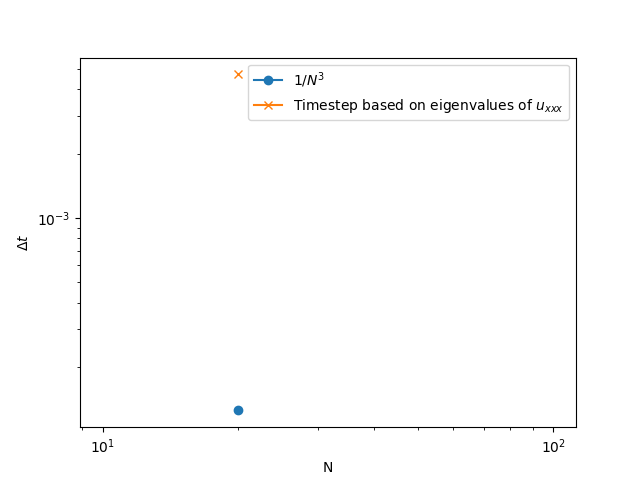
\includegraphics[width=10cm]{Q2Timestep_uxxx.png}
    \caption{Maximum allowable timestep for the Forward Euler discretization of $u_t = -u_{xxx}$ as a function of $N$}
    \label{fig:uxxxtime}
\end{figure}
On the other hand, explicit schemes allow for the possibility to avoid computing the solution to the non linear system of equations corresponding to the $uu_x$ term at every timestep which might become necessary for an implicit method. Furthermore, explicit schemes avoid the cost of computing a matrix inverse in order to solve the coupled system of equations that is obtained for an implicit method.

One also obtains several advantages of using a Collocation spatial discretization as compared to the Fourier Galerkin discretization. The primary advantage lies in the ease of formulation of the $uu_x$ term which can now be easily represented simply as an elementwise product between two vectors $U$ and $\Tilde{D}_1U$. The Fourier Galerkin discretization for the same would require the computation of a convolution matrix in the modal space of Fourier Coefficients which can become a tedious process.

On the other hand, the differentiation matrix corresponding to the Fourier Galerkin discretization of the $u_{xxx}$ term is a diagonal matrix in the modal space. The matrix $\Tilde{D}_3$ for the Collocation discretization is dense and hence, might require more memory space and increase the computational cost for performing matrix vector product for large values of $N$. Furthermore, the use of interpolation operator for the non linear term $uu_x$ introduces the presence of aliasing error in the finally computed solution for the collocation discretization which is not the case for a Fourier Galerkin discretization.

\subsection{(b)}
The implicit formulation of Equation \ref{eq:Q2:explicit_collocation} offers the primary advantage of removing timestep restrictions due to the presence of stiff third derivative operator $u_{xxx}$. For instance, the stability region of the Forward Euler scheme contains the entire left half plane in the Argand diagram of $z = k \lambda$. Hence, one can resort to the usage of much larger timestep values as compared to the explicit schemes. However, the presence of the non linear term $uu_x$ makes the system of discretized equations non linear. Hence, one requires the solution to a non linear system of equations at every timestep which might aggravate the computational cost for large $N$. Furthermore, the requirement to compute the inverse of dense matrices found in the collocation discretization of the spatial operator at every time step can lead to very high computational cost for large values of $N$. 

It is possible to linearize the non linear system of equations and compute the solution to this linearized system at every timestep but one might need very small timestep values to ensure sufficient accuracy which goes against the original objective of reducing the computational cost. 

Implicit schemes usually ensure stability via added dissipation. As also observed in Q1, for large timestep values, the added dissipation has the potential to degrade the solution quality and can be a disadvantage when highly time accurate solutions are desired. 
\subsection{(c)}
As stated in the question, the operator $\mathcal{L}(u)$ is required to be evolved using the implicit Crank Nicolson formulation. The stiff nature of the collocation discretization of the third derivative term found in the original PDE would require severe time stepping restrictions for stability purposes. This makes it suitable for use within the implicit formulation. On the other hand, the operator $\mathcal{N}(u)$ is required to be evolved using the explicit RK2 midpoint formulation. This makes it suitable for use with the non-linear $uu_x$ term which if used with the implicit method would require the solution to a non-linear system of equations at every time step. 

The Strang Splitting time stepping formulation of the collocation discretization presented in Equation \ref{eq:Q2:explicit_collocation} is described further. The Crank Nicolson formulation of $\mathcal{L}(u) = -\Tilde{D}_3 U$ is shown in Equation \ref{eq:strangL}.
\begin{equation}
\begin{aligned}
    & U^{n + 1} = \mathcal{S}_{2, \Delta t} = U^n + \frac{\Delta t}{2}\left( -\Tilde{D}_3 U^n - \Tilde{D}_3 U^{n + 1} \right) \\
    & or \quad U^{n + 1} = \mathcal{S}_{2, \Delta t} = \left( I + \frac{\Delta t \Tilde{D}_3 }{2} \right)^{-1} \left( I - \frac{\Delta t \Tilde{D}_3}{2} \right) U^n
\end{aligned} 
\label{eq:strangL}
\end{equation}

The RK2 midpoint formulation of the non-linear term $\mathcal{N}(u) = 6U \odot \Tilde{D}_1 U$ is described in Equation \ref{eq:strangN}.
\begin{equation}
    \begin{aligned}
        & U^{n + 1} = \mathcal{S}_{1, \Delta t} = U^{n} + \Delta t \mathcal{N}\left( U^n + \frac{\Delta t}{2} 6U^n \odot \Tilde{D}_1 U^n \right) \\
        &  or \quad U^{n + 1} = \mathcal{S}_{1, \Delta t} = U^{n} + 6 \Delta t \left( U^n + \frac{\Delta t}{2} 6U^n \odot \Tilde{D}_1 U^n \right) \odot \left( \Tilde{D}_1 \left( U^n + \frac{\Delta t}{2} 6U^n \odot \Tilde{D}_1 U^n \right) \right)
    \end{aligned}
\label{eq:strangN}
\end{equation}
\subsection{(d)}
Computation of matrices $\Tilde{D}_1$ and $\Tilde{D}_3$ requires the initial computation of the Discrete Fourier Transform Matrix and the inverse Discrete Fourier Transform. Computation of these matrices requires the explicit specification of the Fourier modes. As also stated in Q1, the Fourier modes must be periodic within the specified domain and must be orthonormal. 

Let $\phi_k(x) = c_1 e^{i c_2 k x}$ denote a Fourier Basis mode where $k \in [-N, N]$ and $k \in Z$. All wavelengths corresponding to these modes must be periodic at the domain boundaries. In other words, the period for these modes must be $20$. It is easy to observe that using $c_2 = 2\pi / 20$ leads to $\phi_k(x + 20) = c_1 e^{i2 \pi k (x + 20)/20} = c_1 e^{i2 \pi k x/20} e^{i 2\pi k} = \phi_k(x)$. 

The orthonormality condition requires that $<\phi_k(x), \overline{\phi}_k(x)> = 1$. As a result one arrives at the condition $c_1^2 \int_{x = -10}^{10} e^{i 2\pi k x /20} e^{-i 2\pi k x /20} = 1$ or $c_1 = 1/\sqrt{20}$. Hence, the Fourier basis modes take the form $\phi_k(x) = e^{i 2 \pi k x /20}/\sqrt{20}$.

Assume that the spatial discretization of the domain takes the form $x_j = -10 + 20 \times j/M$ where $j \in [0, M)$, $j \in Z$ and $M = 2N + 1$. 

Let the matrix $V$ represent the matrix corresponding to the Discrete Fourier Transform and let $\Tilde{V}$ represent the matrix corresponding to the Inverse Discrete Fourier Transform. Then, we know that the Discrete Fourier series representation for any variable $u$ is given as $u(x_j) = \sum_{\abs{k} \leq N} \hat{u}_k \phi_k(x_j)$. Hence, the components of the matrix $\Tilde{V}$ given as $\Tilde{v}_{ij}$ can be written as $\Tilde{v}_{jk} = \phi_k(x_j)$. A matrix vector multiplication $U = \Tilde{V} \hat{U}$ will provide the solution values in the physical space given the Fourier modal coefficients in the frequency space. 

Due to orthonormality of Fourier Basis modes, it is possible to write $\hat{u}_k = <u(x), \phi_k(x)>$. As a result, one can derive explicit formula for $\hat{u}_k$ as shown in Equation \ref{eq:Q2_modes}.
\begin{equation}
    \begin{aligned}
        & \hat{u}_k = \frac{1}{\sqrt{20}} \int_{x = -10}^{10} u(x) e^{\frac{-i 2 \pi k x}{20}} dx 
    \end{aligned}
\label{eq:Q2_modes}
\end{equation}

The integral shown in Equation \ref{eq:Q2_modes} needs to be approximated. However, a simple rectangular rule leads to exact computation of the integrals for $\abs{k} \leq N - 1$ as shown in Hesthaven. Furthermore, one observes that $\hat{u}_{-N} = \hat{u}_{N}$. Hence, the modes $\hat{u}_N$ and $\hat{u}_{-N}$ are aliased as also shown in Shen, Tang and Wang. Hence, one resorts to the use of the approximation shown in Equation \ref{eq:Q2_finalmodes}.
\begin{equation}
    \begin{aligned}
        & \hat{u}_k = \frac{1}{\sqrt{20}} \frac{20}{M} \sum_{j = 0}^{M - 1} \frac{u(x_j)}{\Tilde{c}_k} e^{\frac{-i 2 \pi k x_j}{10}} =   \frac{\sqrt{20}}{M} \sum_{j = 0}^{M - 1} \frac{u(x_j)}{\Tilde{c}_k} e^{\frac{-i 2 \pi k x_j}{10}} \\
        & where \quad \Tilde{c}_k = 2 \quad when \quad  k \in \{ -N, N \} \\
        & and \quad  \Tilde{c}_k = 1 \quad when \quad \abs{k} \leq N - 1
    \end{aligned}
    \label{eq:Q2_finalmodes}
\end{equation}
Hence, the components of the matrix $V$ given as $v_{kj}$ can be represented as $v_{kj} = \sqrt{20} e^{-i 2 \pi k x_j/10}/(M \Tilde{c}_k)$. A simple matrix vector multiplication $\hat{U} = VU$ will provide the Fourier modal coefficients in the frequency space.

The diagonal components $d^3_{ij}, d^1_{ij}$ of the Differentiation matrices in the modal space ($D_3$ and $D_1$) are given as $d^3_{kk} = i 2 \pi k /20$ and $d^1_{kk} = (i 2 \pi k /20)^3$. The off-diagonal components are equal to $0$ for these matrices. Hence, the Differentiation matrices in the physical space take the form $\Tilde{D}_3 = \Tilde{V} D_3 V$ and $\Tilde{D}_1 = \Tilde{V} D_1 V$.

Using these matrices, computations were performed for $N = 64$ until $t = 1$. The simulation results are shown in Figure \ref{fig:Q2_N=64,t=1}. The solution result shows a peak at $x = 0$ in the initial condition which moves forward without any change of shape. 
\begin{figure}
    \centering
    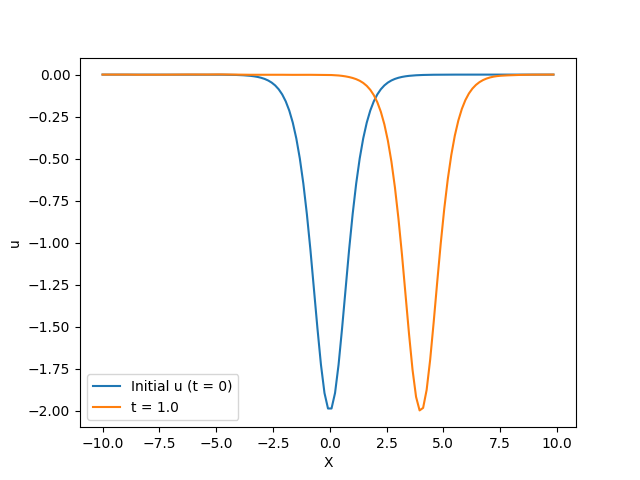
\includegraphics[width = 10cm]{solutionPlot_N=64t = 1.0.png}
    \caption{Solution Plot for the KdV Equation at $t = 1.0$ and $N = 64$}
    \label{fig:Q2_N=64,t=1}
\end{figure}
It turns out that a timestep condition equal to $0.1/max(\abs{\lambda_k})$ provided a stable numerical simulation for $N = 64$ which is a much less severe condition than the one which would have been possible if the timestep restriction was based on $1/max(\abs{\lambda_k^3})$. On the other hand, a non-linear optimization problem was not required for the $uu_x$ term which further alleviates the computational cost for large enough $N$.

Solution results were also plotted for $N = 20$ at $t = 1.0$. It turns out that the same phenomenon was observed where the solution peak at $x = 1.0$ moved forward without any change of shape but it turns out that due to less number of points, the peak was not well resolved and some oscillations were observed for small values of $N$.
\begin{figure}
    \centering
    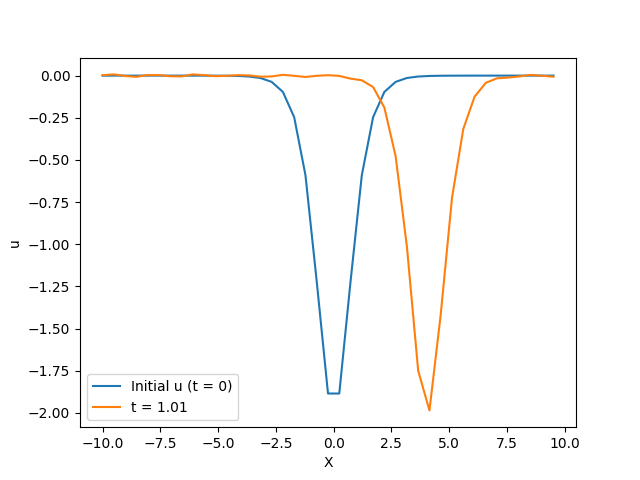
\includegraphics[width = 10cm]{solutionPlot_N=20t = 1.01.png}
    \caption{Solution Plot for the KdV Equation at $t = 1.0$ and $N = 20$}
    \label{fig:Q2_N=64,t=1}
\end{figure}

\section{Appendix}
Simulations were performed to compute the solution of $u_t + sin(2 \pi x)u_x = 0$ at different times using the Fourier Galerkin Scheme presented in Question $1$. The Equation $u_t + sin(2 \pi x)u_x = 0$ could be obtained by simply removing the $u_{xx}$ term for the problem stated in Question $1$. It turns out that the exact solution to the equation involves a discontinuity even when the initial data is smooth $(u(x, 0) = sin(2 \pi x))$. Figure \ref{fig:app:uxplot} shows the Fourier Galerkin solution at different times. \an{This is not true -- the solution actually remains smooth, but the transition region simply becomes smaller and smaller; when it's too small, a truncated Fourier series simply cannot represent such things accurately. The reason you develop oscillations is due to the fact that for the true (infinite-dimensional) solution, those oscillations would be counteracted with oscillations from basis functions outside the Galerkin space. But since those modes are truncated, the oscillations are apparent. (You mention something similar to this below.)}

It is observed that as soon as the discontinuity forms, spurious oscillations are observed. This possibly reflects the lack of positivity for the Fourier Galerkin scheme which shows oscillatory behavior in the presence of discontinuities. This also might possibly reflect that the truncated Fourier series discretization is unable to represent the discontinuous solution as is observed for the truncated Fourier Series expansion for a step function where the spectrum is spread across the entire frequency range.
\begin{figure}
    \centering
    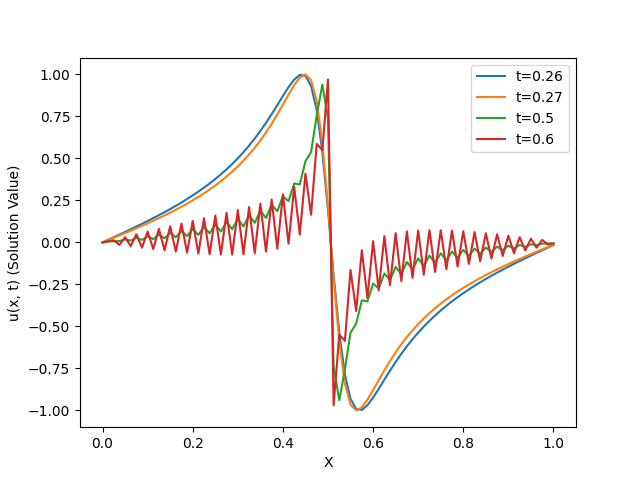
\includegraphics[width=10cm]{uxplot_Q1.png}
    \caption{Fourier Galerkin solution to the Equation $u_t + sin(2 \pi x)u_x = 0$}
    \label{fig:app:uxplot}
\end{figure}
\end{document}
